\begin{minipage}{0.45\linewidth}
    \textbf{Protein fibres:} \textbf{Collagen} and \textbf{Elastin}      provide \textbf{strength} and \textbf{elasticity}
\end{minipage}
\begin{minipage}{0.45\linewidth}
    \textbf{Glycoproteins:} \textbf{Fibronectin} and \textbf{Laminin}      provide \textbf{adhesion} and \textbf{signaling}
\end{minipage}
\begin{minipage}{0.45\linewidth}
    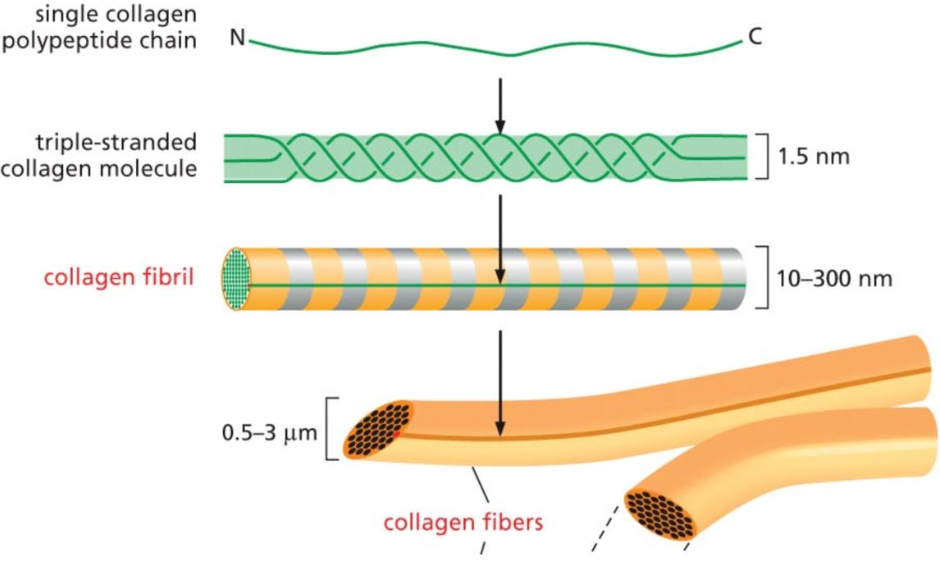
\includegraphics[width=35mm]{src/Images/collagen.png}
\end{minipage}
\begin{minipage}{0.45\linewidth}
    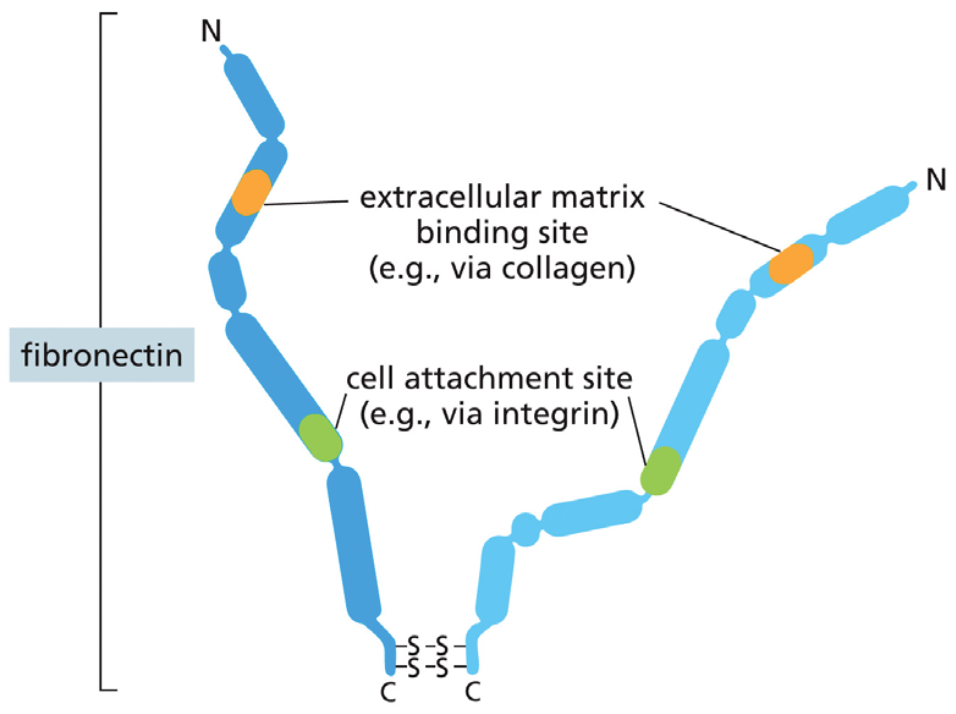
\includegraphics[width=30mm]{src/Images/glycoprotein.png}
\end{minipage}\\

Glycosaminoglycans (GAGs) and Proteoglycans:\\

\begin{itemize}
    \item \textbf{Linear}, \textbf{rigid} polysaccharide \textbf{chains} → form large volumes of porous gels
    \item They carry \textbf{negative charges} → \textbf{retention of water}
    \item Often covalently linked to protein cores called proteoglycans that also provides lubrication
    \item \textbf{Resistance to compression}
\end{itemize}

All components are \textbf{produced} and matured \textbf{in the cells} then secreted in extracellular environment\\
→ Cells engineer their local extracellular matrix
